% !TEX root = ../Main.tex
\subsection{Freidberg's simple reactor model}
In the \nth{5} chapter of the textbook by Freidberg\cite{freidberg_plasma_2007}, he makes a simple model for designing a fusion reactor power plant.
The model uses simple geometric and electromagnetic assumptions with little involvement of plasma physics. The variables put into the model are shown in \cref{VFR}.
\begin{table}
	\centering
	\begin{tabular}{lr}
		\toprule
		Symbol                         & Quantity                                                                                 \\
		\midrule
		\(n_\mathrm{flux \ fraction}\) & n flux in breeder end/n flux in breeder start \(\bqty{1}\)                                \\
		\(C_F\)                        & Fixed cost proportionality constant \(\bqty{\$}\)                                         \\
		\(C_I\)                        & Nuclear island cost proportionality constant \(\bqty{\$\cdot\si{\watt\per\meter\cubed}}\) \\
		\(P_E\)                        & Desired output power \(\bqty{\si{\mega\watt}}\)                                          \\
		\(P_W\)                        & Maximum wall load \(\bqty{\si{\mega\watt\per\meter\squared}}\)                           \\
		\(B_{\max}\)                   & Magnetic field at the edge of the coil \(\bqty{\si{\tesla}}\)                            \\
		\(\sigma_{\max}\)              & Tensile strength of the magnetic field coils \(\bqty{\si{\atm}}\)                        \\
		\(\eta_t\)                     & Energy conversion efficiency \(\bqty{1}\)                                                 \\
		\bottomrule
	\end{tabular}
	\caption{Variables in the Freidberg's model}
	\label{VFR}
\end{table}
\cref{QFR} shows the output quantities from the model.
\begin{table}
	\centering
	\begin{tabular}{llr}
		\toprule
		Symbol                    & Quantity                                                       & Obtained values                  \\
		\midrule
		\(b\)                     & Blanket-and-shield thickness                                   & \SI{1.2037}{\meter}              \\
		\(c\)                     & Magnet coil thickness                                          & \SI{0.7993}{\meter}              \\
		\(a\)                     & Minor radius                                                   & \SI{2.0098}{\meter}              \\
		\(R_0\)                   & Major radius                                                   & \SI{4.9583}{\meter}              \\
		\(A\)                     & Aspect ratio                                                   & 2.4670                           \\
		\(A_p\)                   & Plasma surface                                                 & \SI{393.4152}{\meter\squared}    \\
		\(V_p\)                   & Plasma volume                                                  & \SI{395.3509}{\meter\cubed}      \\
		\(P_\mathrm{dens}\)       & Power density                                                  & \SI{4.9685e06}{\watt\per\meter}  \\
		\(p\)                     & Plasma pressure                                                & \SI{7.3672e05}{\pascal}          \\
		\(n\)                     & Particle density                                               & \SI{1.5327e20}{\per\meter\cubed} \\
		\(B_0\)                   & Magnetic field at magnetic axis                                & \SI{4.5744}{\tesla}              \\
		\(\beta\)                 & Normalised plasma pressure                                     & 8.85\%                           \\
		\(\tau_{E_\mathrm{min}}\) & Min confinement time for \(\pqty{p\times\tau_E}_\mathrm{min}\) & \SI{1.1415}{\second}             \\
		\bottomrule
	\end{tabular}
	\caption{Output quantities in the model in Freidberg's\cite{freidberg_plasma_2007} along with the obtained values when inserting the parameters from \cref{Inputparam}}
	\label{QFR}
\end{table}
This model has been implemented in a Matlab script provided for the course. The script is shown included in \cref{tokamakDTU_asign_1}.
As an example, the model is run with the following parameters:
\begin{alignat}{3}
	n_\mathrm{flux \ fraction} & = 0.01                                 & \quad P_E      & = \SI{1000}{\mega\watt} \nonumber       \\
	P_W                        & = \SI{4}{\mega\watt\per\meter\squared} & \quad B_{\max} & = \SI{13}{\tesla}    \label{Inputparam} \\
	\sigma_{\max}              & = \SI{3000}{\atm}                      & \quad \eta_t   & = 0.4 \nonumber
\end{alignat}
Note that \(C_F\) and \(C_I\) has been omitted as these serve no purpose for this assignment. It is not of interest how expensive the plant will be. Rather the geometries and physical quantities are of interest.
The results from the model is given in \cref{QFR}.


\subsection{Model sensitivity}


At this point Freidberg has provided a model that produce some reasonable results for a power plant. It could be interesting to see how this model behaves when some vital parameters are changed. In the last section the model used the parameters shown in \cref{Inputparam}. In \cref{variparam} are listed some parameter ranges.
\begin{alignat}{3}
	P_E &: \SIrange{500}{1000}{\mega\watt} & \quad P_W &: \SIrange{0}{10}{\mega\watt\per\meter\squared}\nonumber\\
	B_{\max} &: \SIrange{0}{20}{\tesla} & \quad \sigma_{\max} &: \SIrange{2000}{5000}{\atm}\label{variparam}
\end{alignat}
\cref{IterateTokamakDTU} includes Matlab code that does the following:
\begin{enumerate}
	\item Take a variable range from \cref{variparam}.
	\item Set all other input parameters as in \cref{Inputparam}.
	\item Plot the model outputs as functions of the variable range.
	\item Repeat with another range from \cref{variparam}.
\end{enumerate}
The iteration showed some interesting breakdowns in the model. When varying the desired power output there was a breakdown in magnetic field strength at the magnetic axis as well as in the normalised plasma pressure. This is shown in \cref{PE}.
\begin{figure}
	\centering
  \begin{subfigure}[b]{.46\textwidth}
    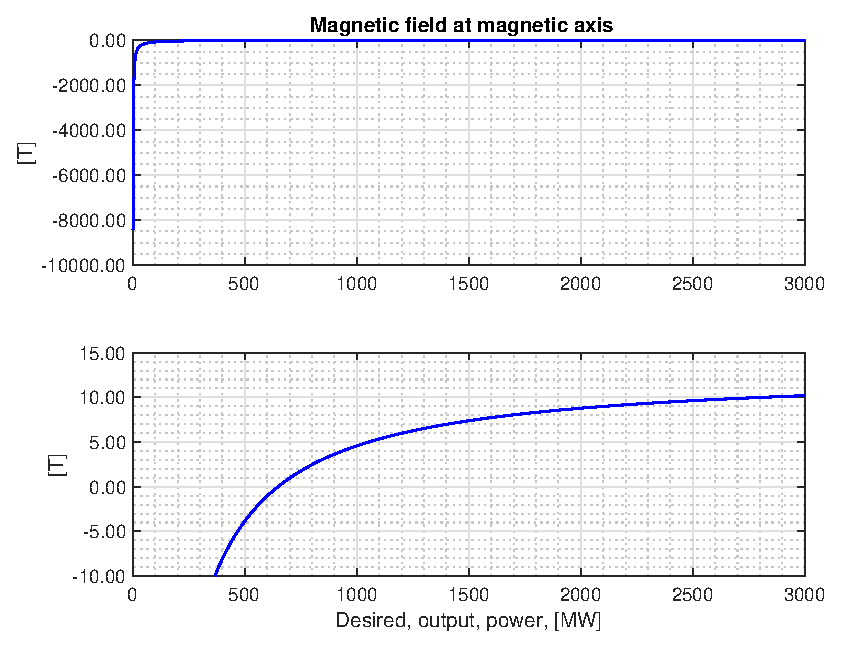
\includegraphics[width=\textwidth]{MatlabFigures/PE/f7.eps}
    \caption{The magnetic field at magnetic axis\vspace{\baselineskip}}
    \label{PEM}
  \end{subfigure}
  ~
  \begin{subfigure}[b]{.45\textwidth}
    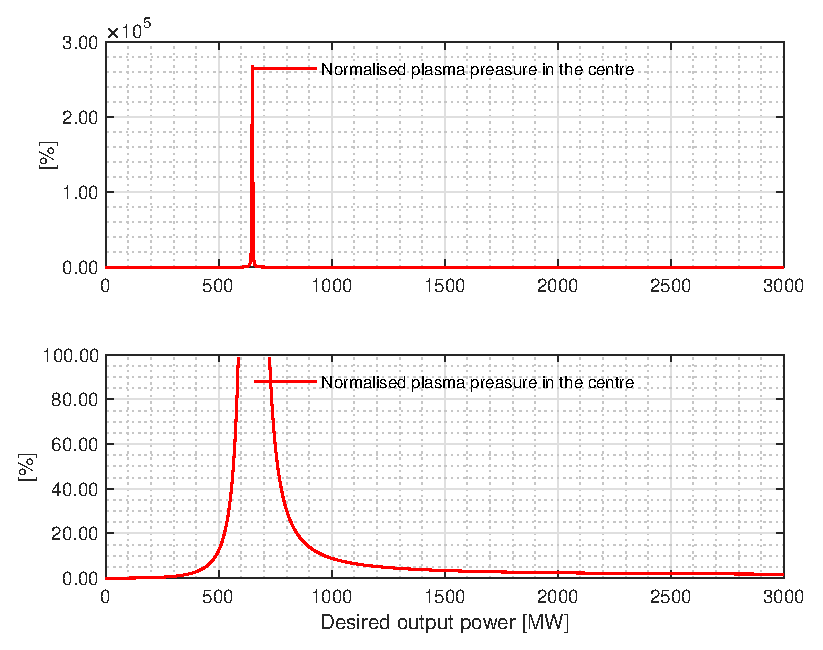
\includegraphics[width=\textwidth]{MatlabFigures/PE/f8.eps}
    \caption{The normalised plasma pressure in the centre}
    \label{PEB}
  \end{subfigure}
	\caption{Model breakdown when iterating over desired power output.}
	\label{PE}
\end{figure}
In this case, limits for what is physically possible broke and in these cases the model is unusable.
The full gallery of model output is found in \cref{ITFR}.
\subsection{Elliptic Cross section}
Freidberg's model assume a circular cross section of the plasma. In reality this is not the case. We will now make a more realistic, yet still approximate reactor for an elliptic plasma cross section.
In describing the geometry one refers to the elongation ratio:
\begin{align}
	\kappa = \frac{a_{\max}}{a_{\min}}
\end{align}
With $a_{\max}$ the major radius and $a_{\min}$ the minor radius of the ellipse. This parameter ensures a true elliptic cross section as defined by the equation,
\begin{align}
	\frac{x^2}{a_{\max}}+\frac{y^2}{a_{\min}} = 1
\end{align}
which can be parameterised as
\begin{align}
	\mqty[x_1 \\y_1] &= \mqty[a_{\min}\cos{\phi}\\\kappa a_{\min}\sin{\phi}]
	\label{eq:inner_ellipse}
\end{align}
Meanwhile the blanket must be implemented as an ellipse or swelled ellipse. The true ellipse results in a thickness difference throughout the blanket, while the second model results in a blanket of equal thickness throughout. To this, the choice of implementing the blanket as a true ellipse has been made, since it simplifies derivations a bit. Note however, that keeping a constant thickness is the preferable option as it will reduce the engineering volume and hence the cost of the machine.\\
The outer layer is parameterised
\begin{align}
	\mqty[x_2 \\y_2] &= \mqty[\pqty{b+a_{\min}}\cos{\phi}\\\kappa \pqty{b+a_{\min}}\sin{\phi}]
	\label{eq:outer_ellipse}
\end{align}
with $b$ the blanket thickness at the minor ellipse axis. Choosing for now, $a_{\min}=2$, $\kappa=2$ and $b=1.2$, \cref{eq:inner_ellipse} and \cref{eq:outer_ellipse} are plotted on Figure \cref{ShTh} along with the variation in thickness of the blanket.
\begin{wrapfigure}[14]{r}{.4\textwidth}
	\vspace{3mm}
	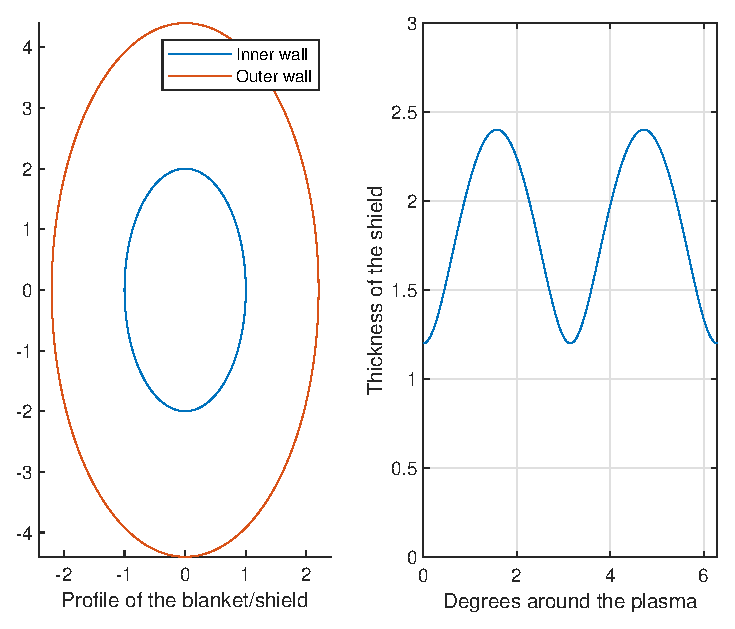
\includegraphics[width=.4\textwidth]{MatlabFigures/ShieldThickness/ShieldThickness.eps}
	\caption{The profile of the blanket-and-shield and the thickness as a function of the angle around origin, \(\phi\).}
	\label{ShTh}
\end{wrapfigure}
Given \cref{eq:inner_ellipse} and \cref{eq:outer_ellipse}, the engineering volume can easily be derived if $c\,\cos(\phi)$ and $\kappa\, c\,\sin(\phi)$ is added to the x and y-direction in \cref{eq:outer_ellipse} respectively, where $c$ is the minimum thickness of the magnetic coils that provide the toroidal field. \\
The cross sectional area of an ellipse is $A_{\si{e}}=\pi\, a_{\min}\, a_{\max}$ so the engineered volume becomes
\begin{align}
	V_{\si{I}} & =2\,\pi\, R_{0}\,(A_{\si{e,outer}}-A_{\si{e,inner}}) \nonumber                        \\
	           & = 2\,\pi^{2}\, R_{0}\,\left(\left(a_{\min}+b+c\right)^{2}-a_{\min}^{2}\right)\,\kappa
	\label{eq:engineered_volume}
\end{align}
and the plasma volume is similarly calculated as $V_{\si{P}}=2\,\pi^2\, R_{0}\,\kappa\, a_{\min}^{2}$. The plasma surface area is a bit more tricky, but it can be approximated as
\begin{align}
	S_{\si{p}}=2\,\pi\, R_{0}\,\pi\,(3\,(a_{\min}+\kappa\, a_{\min})-\sqrt{(3\, a_{\min}+\kappa\, a_{\min})\,(a_{\min}+3\,\kappa\, a_{\min})})
\end{align}
Using the same arguments as in the book, the B-field in the centre is surprisingly unchanged when going to the elliptical model. Now c is also approximated, or rather overestimated using a slight change to Eq. (5.24) in the textbook. Since the force grows with $a_{\min}$, inserting $\kappa\, a_{\min}$ instead yields an overestimation on the vertical force on the magnet. The tensile forces are the same, so the force balance leads to
\begin{align}
	c=\frac{2\,\xi}{1-\xi}(\kappa\, a+b)
\end{align}
with $\xi=B_{si{c}}^2/4\,\mu_{0}\,\sigma_{\si{max}}$. These new equations are inserted in the code. The results are displayed in \ref{tab:ellip_output}. The plasma volume and surface area is of course increased as the plasma was made higher. This of course also results in a decreased power density. Overall, parameters such as $B_{0}$, $\beta$ and $\tau_{\si{E_{\min}}}$ while changing a bit, they were not changed significantly.
\begin{table}
	\centering
	\begin{tabular}{llr}
		\toprule
		Symbol                    & Quantity                                                       & Obtained values                  \\
		\midrule
		\(b\)                     & Blanket-and-shield thickness                                   & \SI{1.2037}{\meter}              \\
		\(c\)                     & Magnet coil thickness                                          & \SI{1.2992}{\meter}              \\
		\(a\)                     & Minor radius                                                   & \SI{2.0098}{\meter}              \\
		\(R_0\)                   & Major radius                                                   & \SI{4.9583}{\meter}              \\
		\(A\)                     & Aspect ratio                                                   & 2.4670                           \\
		\(A_p\)                   & Plasma surface                                                 & \SI{608.7415}{\meter\squared}    \\
		\(V_p\)                   & Plasma volume                                                  & \SI{793.4534}{\meter\cubed}      \\
		\(P_\mathrm{dens}\)       & Power density                                                  & \SI{2.4756e06}{\watt\per\meter}  \\
		\(p\)                     & Plasma pressure                                                & \SI{5.2003e05}{\pascal}          \\
		\(n\)                     & Particle density                                               & \SI{1.0819e20}{\per\meter\cubed} \\
		\(B_0\)                   & Magnetic field at magnetic axis                                & \SI{4.6037}{\tesla}              \\
		\(\beta\)                 & Normalised plasma pressure                                     & 6.17\%                           \\
		\(\tau_{E_\mathrm{min}}\) & Min confinement time for \(\pqty{p\times\tau_E}_\mathrm{min}\) & \SI{1.6172}{\second}             \\
		\bottomrule
	\end{tabular}
	\caption{Output quantities from the elliptical model}
	\label{tab:ellip_output}
\end{table}
\subsection{Main parameters for DEMO}
Setting $P_{\si{E}}=2000$ in the elliptical model yields the output parameters seen in  \cref{tab:DEMO}. Since $R_{0}$ is directly proportional to the electric power, it increases linearly. The other geometric output parameters regarding areas and volumes also increase as a result. $\beta$ has decreased a lot, so the plasma is not confined effectively in DEMO.
\begin{table}
	\centering
	\begin{tabular}{llr}
		\toprule
		Symbol                    & Quantity                                                       & Obtained values                  \\
		\midrule
		\(b\)                     & Blanket-and-shield thickness                                   & \SI{1.2037}{\meter}              \\
		\(c\)                     & Magnet coil thickness                                          & \SI{1.2992}{\meter}              \\
		\(a\)                     & Minor radius                                                   & \SI{2.0098}{\meter}              \\
		\(R_0\)                   & Major radius                                                   & \SI{9.9510}{\meter}              \\
		\(A\)                     & Aspect ratio                                                   & 4.9512                           \\
		\(A_p\)                   & Plasma surface                                                 & \SI{1.21175e03}{\meter\squared}  \\
		\(V_p\)                   & Plasma volume                                                  & \SI{1.5869e03}{\meter\cubed}     \\
		\(P_\mathrm{dens}\)       & Power density                                                  & \SI{2.4756e06}{\watt\per\meter}  \\
		\(p\)                     & Plasma pressure                                                & \SI{5.2003e05}{\pascal}          \\
		\(n\)                     & Particle density                                               & \SI{1.0819e20}{\per\meter\cubed} \\
		\(B_0\)                   & Magnetic field at magnetic axis                                & \SI{8.8018}{\tesla}              \\
		\(\beta\)                 & Normalised plasma pressure                                     & 1.69\%                           \\
		\(\tau_{E_\mathrm{min}}\) & Min confinement time for \(\pqty{p\times\tau_E}_\mathrm{min}\) & \SI{1.6172}{\second}             \\
		\bottomrule
	\end{tabular}
	\caption{Output quantities for DEMO using the elliptical model with $P_{\si{E}}=2\si{GW}$}
	\label{tab:DEMO}
\end{table}
\subsection{Designs for DEMO}
With $P_{\si{E}}$, $\kappa=2$ and $A=R_{0}/a_{\min}=3\Leftrightarrow R_{0}=3\, a_{\min}$. This is implemented in the code and the results are displayed in \ref{tab:DEMO2}. $\beta$ has increased a bit but only to $4.55\%$. $R_{0}$ has been forced down, so the plasma volume etc. has decreased as well. Overall it seems like a smaller $R_{0}$ while keeping $a_{min}$ fixed is an improvement. Or in other words, $A=3$ is more desirable than $A\approx 5$.
\begin{table}
	\centering
	\begin{tabular}{llr}
		\toprule
		Symbol                    & Quantity                                                       & Obtained values                  \\
		\midrule
		\(b\)                     & Blanket-and-shield thickness                                   & \SI{1.2037}{\meter}              \\
		\(c\)                     & Magnet coil thickness                                          & \SI{1.2992}{\meter}              \\
		\(a\)                     & Minor radius                                                   & \SI{2.0098}{\meter}              \\
		\(R_0\)                   & Major radius                                                   & \SI{6.0295}{\meter}              \\
		\(A\)                     & Aspect ratio                                                   & 3                                \\
		\(A_p\)                   & Plasma surface                                                 & \SI{737.6961}{\meter\squared}    \\
		\(V_p\)                   & Plasma volume                                                  & \SI{961.5370}{\meter\cubed}      \\
		\(P_\mathrm{dens}\)       & Power density                                                  & \SI{4.0857e06}{\watt\per\meter}  \\
		\(p\)                     & Plasma pressure                                                & \SI{6.6807e05}{\pascal}          \\
		\(n\)                     & Particle density                                               & \SI{1.3899e20}{\per\meter\cubed} \\
		\(B_0\)                   & Magnetic field at magnetic axis                                & \SI{6.0714}{\tesla}              \\
		\(\beta\)                 & Normalised plasma pressure                                     & 4.55\%                           \\
		\(\tau_{E_\mathrm{min}}\) & Min confinement time for \(\pqty{p\times\tau_E}_\mathrm{min}\) & \SI{1.2588}{\second}             \\
		\bottomrule
	\end{tabular}
	\caption{Output quantities for DEMO using the elliptical model with $P_{\si{E}}=2$, $\kappa=2$ and $A=3$.}
	\label{tab:DEMO2}
\end{table}
\subsection{\textit{A} and \mathinhead{\kappa}{\kappa} as free parameters}
Designing the tokamak with $\kappa$ and $A$ as free parameters has led us to try and maximise profitability from $V_{P}/A_{P}$ and $\beta$. Profitability in this context means that increasing the size of the tokamak leads to an increase in these parameters. However, there is a point when the change vs increase in size becomes constant. This means that we do not profit from increasing the size any longer. \\
$V_{\mathrm{P}}$ and $A_{\mathrm{P}}$ were calculated earlier so
\begin{align}
	\frac{V_{\si{P}}}{A_{\si{P}}} & =\frac{2\,\pi\, R_{0}\,\kappa\, a_{\min}^{2}}{2\,\pi\, R_{0}\,\pi\, (3\,(a+\kappa\, a_{\min})-\sqrt{(3\, a_{\min}+\kappa\, a_{\min})\,(a+3\,\kappa\, a_{\min})})} \nonumber \\
	                              & =\frac{\kappa\, a_{\min}}{\pi\,(3+3\,\kappa-\sqrt{3+\kappa}\,\sqrt{1+3\,\kappa})}
\end{align}
The expression scales linearly with $a_{min}$ so we set it equal to \SI{1}{\meter} since it has no effect on the choice of $\kappa$. Differentiating with respect to $\kappa$ and plotting is done, with the results shown in \cref{kappa_change}. Considering the figure, $\kappa=2.5$ is chosen as the change is close enough to zero given this value.\\
Now work will be done towards choosing a value for $A$. First, for geometric reasons, a minimum $R_{0}$ is calculated. It is simply $R_{0}=a_{\min}+b+c$ where $a_{min}$ is to be determined, $b=1.2\si{m}$ and $c=\frac{2\,\xi}{1-\xi}(\kappa\, a_{\min}+b)$. Meanwhile $A$ is chosen to optimise $\beta$. Inserting $R_{0}$ into $B_{0}$ in the textbook yields
\begin{align}
	B_{0}=\frac{2\,\xi\,(\kappa\, a_{\min}+b)\, B_{max}}{((2\,\kappa-1)\, a_{\min}+a+b)}=\frac{178.75\, a_{\min}+85.8}{55.5+36\, a_{\min}}
\end{align}
Where units has been disregarded and $\xi=0.11$, $b=1.2$, $\kappa=2.5$ and $B_{\si{max}}=13$ has been inserted. Meanwhile, inserting the textbook's expression for $P_{\si{dens}}$ into the expression for $p$ and inserting the input parameters yields
\begin{align}
	p=\SI{1.042e6}{}\,\sqrt{\frac{1}{\kappa\, a_{\min}}}
\end{align}
Thus \(\beta\) becomes
\begin{align}
	\beta=\frac{2148\,(a_{\min}+1.542)^{2}}{\sqrt{a_{\min}}\,(178.8\, a_{\min}+85.8)^{2}}
\end{align}
This function is plotted in \cref{beta_vs_a}, and for $\beta=10\%$ $a=\SI{1.938}{\meter})$ is achieved. Therefore $(R_{0}=\SI{1.9378}{\meter}+\SI{1.2}{\meter}+2\cdot 0.11/(1-0.11)\cdot 2.5\cdot \SI{1.938}{\meter}+\SI{1.2}{\meter}=\SI{4.632}{\meter})$ which means $A=\SI{4.632}{\meter}/\SI{1.938}{\meter}=\SI{2.390}{\meter}$
\begin{figure}
	\centering
	\begin{subfigure}[b]{.40\textwidth}
		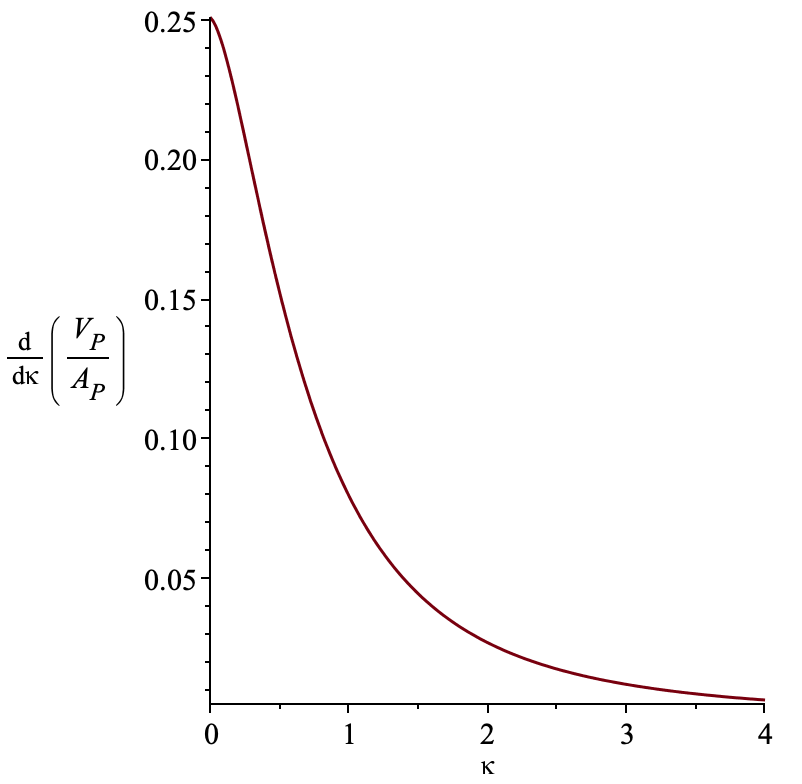
\includegraphics[width=\textwidth]{Figures/kappa_change.png}
		\caption{The change in the ratio between plasma volume per plasma surface area.}
		\label{kappa_change}
	\end{subfigure}
	~
	\begin{subfigure}[b]{.40\textwidth}
		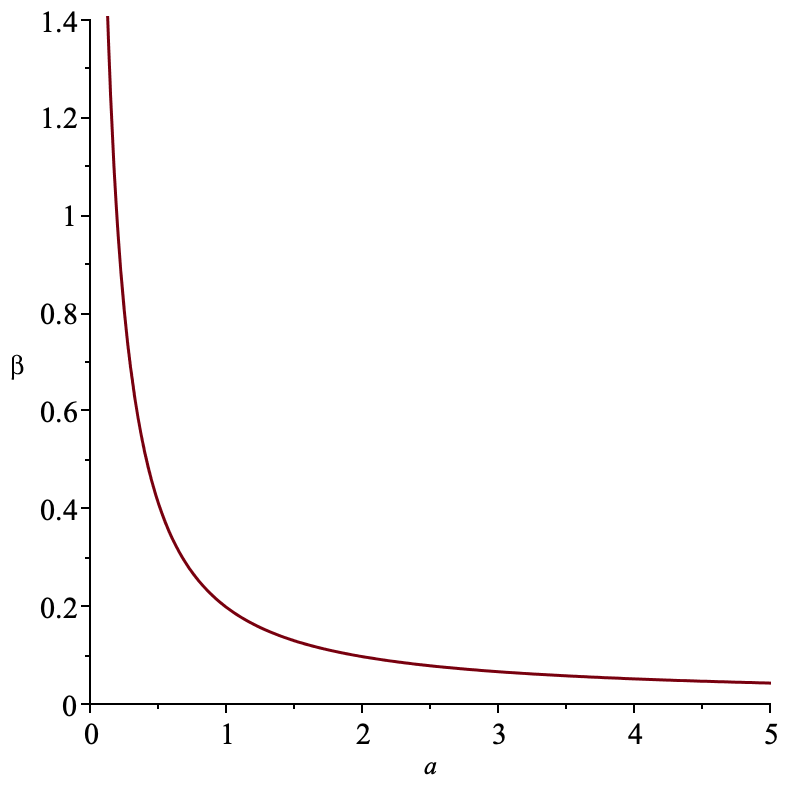
\includegraphics[width=\textwidth]{Figures/beta_vs_a.png}
		\caption{The normalised plasma pressure as a function of the minor radius.\vspace{\baselineskip}}
		\label{beta_vs_a}
	\end{subfigure}
	\caption{}
	\label{A_kappa}
\end{figure}
\begin{table}
	\centering
	\begin{tabular}{llr}
		\toprule
		Symbol                    & Quantity                                                       & Obtained values                \\
		\midrule
		\(b\)                     & Blanket-and-shield thickness                                   & \SI{1.20}{\meter}              \\
		\(c\)                     & Magnet coil thickness                                          & \SI{1.30}{\meter}              \\
		\(a\)                     & Minor radius                                                   & \SI{2.01}{\meter}              \\
		\(R_0\)                   & Major radius                                                   & \SI{4.632}{\meter}              \\
		\(A\)                     & Aspect ratio                                                   & 2.390                           \\
		\(A_p\)                   & Plasma surface                                                 & \SI{630}{\meter\squared}       \\
		\(V_p\)                   & Plasma volume                                                  & \SI{414}{\meter\cubed}         \\
		\(P_\mathrm{dens}\)       & Power density                                                  & \SI{9.49e06}{\watt\per\meter}  \\
		\(p\)                     & Plasma pressure                                                & \SI{1.02e05}{\pascal}          \\
		\(n\)                     & Particle density                                               & \SI{2.12e20}{\per\meter\cubed} \\
		\(B_0\)                   & Magnetic field at magnetic axis                                & \SI{-3.09}{\tesla}             \\
		\(\beta\)                 & Normalised plasma pressure                                     & 26.9\%                         \\
		\(\tau_{E_\mathrm{min}}\) & Min confinement time for \(\pqty{p\times\tau_E}_\mathrm{min}\) & \SI{1.26}{\second}             \\
		\bottomrule
	\end{tabular}
	\caption{Output quantities for the elliptical model after $\beta$ and $A$ has been optimised}
	\label{tab:DEMO3}
\end{table}
